\section{Bevezetés}

A FlockWave szoftver ötlete a drónok monitorozására és vezérlésére készült
régebbi GroundControl nevű parancssori eszköz (lásd \ref{fig:groundcontrol}.
ábra) grafikus megjelenítéssel rendelkező megoldásra történő leváltásának
céljával fogalmazódott meg. Ennek az ötletnek a megvalósítási folyamatába
kapcsolódtam be még abban a kezdeti szakaszban, amikor a program körülbelül csak
a drónok pozícióját tartalmazó szerverről érkező csomagok feldolgozására és az
ezekből származó adatok alapján történő térképen való megjelenítésére volt
alkalmas.

\begin{figure}[h!]
  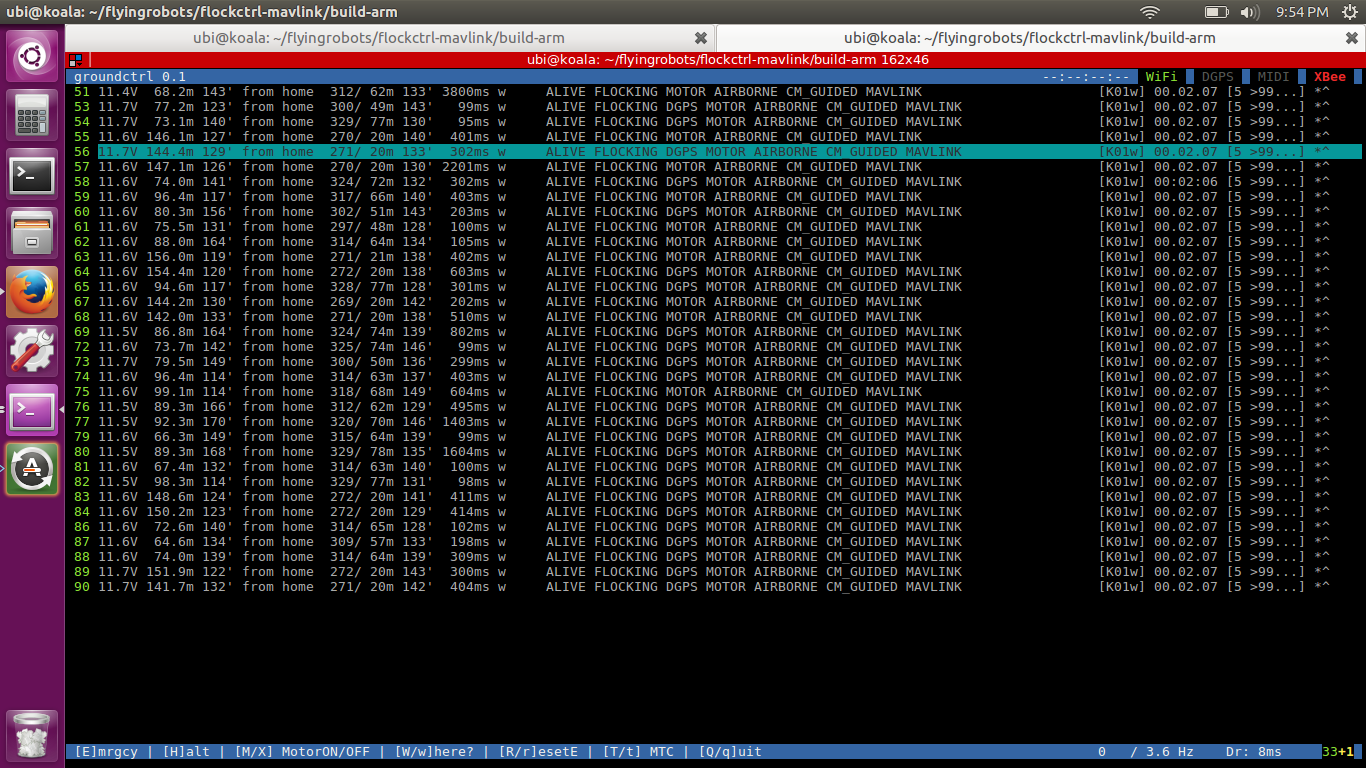
\includegraphics[width=\textwidth]{groundcontrol.png}
  \caption{Képernyőfotó a lecserélésre szánt régi karakteres kezelőfelületről}
  \label{fig:groundcontrol}
\end{figure}

\noindent Ekkor lett a feladatom a rendszer további kiegészítő funkciókkal
történő ellátása. Ezek közül néhányat mutatok be kiemelve ebben a
szakdolgozatban.
